%====================================================================================
\section{Variables Dummy}  
%====================================================================================

\begin{frame}{Variables Dummy}
	\begin{itemize}
		\item Una variable dummy es una variable que toma solo uno de dos valores: 1 ó 0. De ahí­ que también se le conozca como variables
		binarias.
		\item Ejemplos de ello son el género: (=1 si es mujer y cero en otro caso), el ámbito geográfico (=1 si la persona vive en el área rural y
		cero si vive en el área urbana), etc
		\item Otros nombres que son usados para este tipo de variables son: variables ficticias o variables dicotómicas
	\end{itemize}
\end{frame}

%------------------------------------------------------------------------------------
\subsection{Variable dummy como variable independiente}
%------------------------------------------------------------------------------------
\begin{frame}{Variable dummy como variable independiente}
	\begin{itemize}
		\item Sea un modelo regresión lineal múltiple con $y$ y $x$ siendo variables continuas y $d$ una variable dummy:. 
		\pause
				$$y=\beta_{0}+\delta_{0}d+\beta_{1}x+u$$ 
		\pause
		\item Lo cual puede ser interpretado como un cambio en el intercepto: 
		\pause
		\begin{itemize}
			\item Si $d=0$, entonces $y=\beta_{0}+\beta_{1}x+u$
			\item Si $d=1$, entonces $y=(\beta_{0}+\delta_{0})+\beta_{1}x+u$
			\pause
		\end{itemize}
	\end{itemize}
\end{frame}
%---------------------------------------------------
\begin{frame}{Variable dummy como variable independiente}
	Gráficamente y cuando $\delta_{0}>0$ se tendría:
    	\begin{figure}[H]
	    	\begin{centering}
	    	  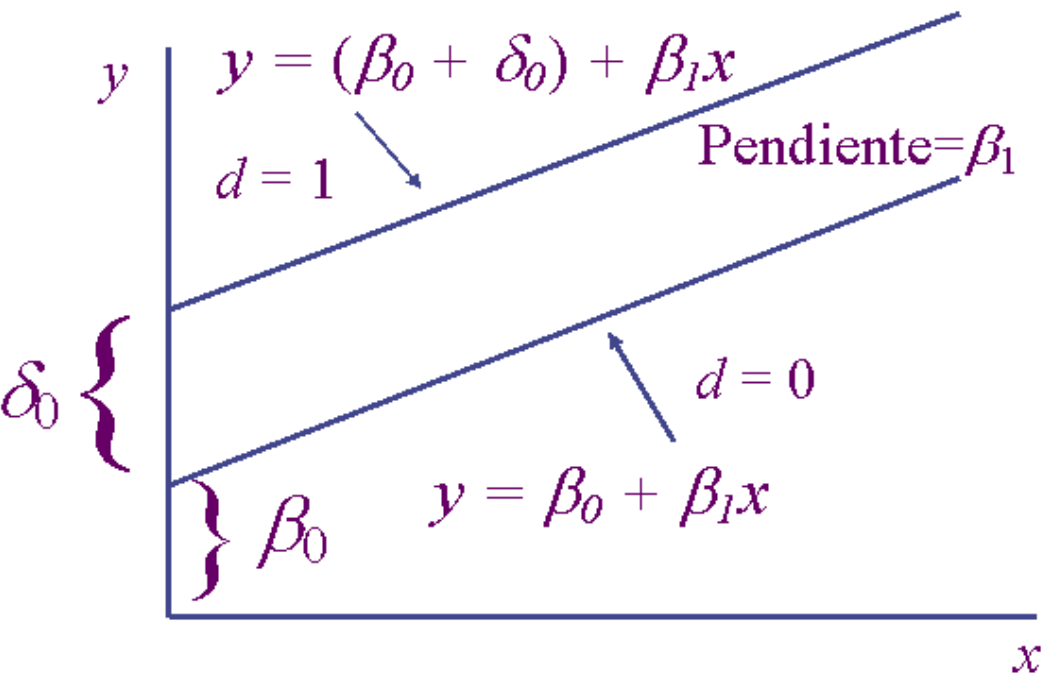
\includegraphics[width = 0.8\linewidth]{fig/dummy1.png}
	    	\end{centering}
    	\end{figure}
\end{frame}
%---------------------------------------------------
\begin{frame}{Variable dummy como variable independiente}
	\begin{itemize}
		\item La variable categórica 'Género' tiene dos categorí­as (Hombre y mujer) Porqué solo se considera una dicotómica en los modelos de
		regresión: $y=\beta_{0}+\delta_{0}Mujer+\beta_{1}x+u$ y no se hace esto: $y=\beta_{0}+\delta_{0}Mujer+\delta_{1}Hombre+\beta_{1}x+u$
		\pause
		\item Porque si se hiciera se tendrí­a el problema de multicolinealidad perfecta: $Hombre+Mujer=1$
		\pause
		\item Es decir, de una variable categórica que tiene dos categoría, solo una se debe incluir en el modelo de regresión. En general, si la
		variable tiene $N$ categoría, el modelo de regresión debería contar con $N-1$ variables dicotómicas.
		\pause 
		\item Dicotómica en STATA: \colorbox{codegray}{\texttt{\textcolor{codeblue}{gen} mujer=sexo==2}} (Crea la dicotómica 'mujer')
	\end{itemize}
\end{frame}
%---------------------------------------------------
\begin{frame}{Variable dummy como variable independiente}
	\begin{itemize}
		\item Así, si se quisiera saber si existe diferencia en los ingresos entre las 13 regiones de Chile la ecuación de Mincer debería tener 12
		dicotómicas, cada una representando a una región. La categorí­a no incluida se conoce como la categoría base y su impacto vendría a ser dado
		por el intercepto de la regresión.
		\pause 
		\item En Stata una forma rápida de crear dicotómicas, una para cada categoría es: \colorbox{codegray}{\texttt{\textcolor{codeblue}{tab} region,g(jose)}} (crea las dicotómicas: 'jose1', 'jose2', ..., 'jose13')
		\pause
		\item En el trabajo aplicado también se suele convertir una variable continua en dicotómica. Por ejemplo convertir la variable edad
		(continua) en una variable categórica que identifica a los jóvenes y a los adultos.
		\pause
		\item En STATA lo anterior se podría hacer del siguiente modo:\\ \colorbox{codegray}{\texttt{\textcolor{codeblue}{gen} joven=edad<31}}
	\end{itemize}
\end{frame}

%------------------------------------------------------------------------------------
\subsection{Términos de interacción entre dicotómicas}
%------------------------------------------------------------------------------------
\begin{frame}{Términos de interacción entre dicotómicas}
	\begin{itemize}
		\item Consiste en incluir la multiplicación de variables dicotómicas en la regresión.
		\pause
		\item Así, si se tienen las variables dicotómicas: mujer y rural; una variable dicotómica que se puede incluir es mujer*rural
		\pause
		\item $y=\beta_{0}+\beta_{1}mujer*rural$, con las siguientes posibilidades:
		\pause
		\begin{itemize}
			\item mujer=0 y rural=0; entonces $y=\beta_{0}$
			\item mujer=1 y rural=1; entonces $y=\beta_{0}+\beta_{1}$
			\item mujer=0 y rural=1; entonces $y=\beta_{0}$
			\item mujer=1 y rural=0; entonces $y=\beta_{0}$
		\end{itemize}
	\end{itemize}
\end{frame}
%---------------------------------------------------
\begin{frame}{Términos de interacción entre dicotómicas}
	\begin{itemize}
		\item Hasta el momento todas las dicotómicas vistas solo provocan cambios en los interceptos
		\pause
		\item Es posible modelar cambios en las pendientes de la siguiente manera: $y=\beta_{0}+\beta_{1}x+\delta_{1}*x*mujer+u$:
		\begin{itemize}
			\item mujer=0; $y=\beta_{0}+\beta_{1}x++u$
			\item mujer=1; $y=\beta_{0}+(\beta_{1}+\delta_{1})x+u$
		\end{itemize}
		\pause
		\item Aunque en general se podrí­a modelar cambio en la pendiente y en el intercepto a la vez: $y=\beta_{0}+\delta_{0}mujer+\beta_{1}x*mujer+\delta_{1}*x*mujer+u$
		\begin{itemize}
			\item mujer=0; $y=\beta_{0}+\beta_{1}x++u$
			\item mujer=1; $y=(\beta_{0}+\delta_{0})+(\beta_{1}+\delta_{1})x+u$
		\end{itemize}
	\end{itemize}
\end{frame}
%---------------------------------------------------
\begin{frame}{Términos de interacción entre dicotómicas}
	Gráficamente y cuando $\delta_{0}>0$ y $\delta_{1}<0$ se tendrí­a:
    	\begin{figure}[H]
    		\begin{centering}
    		  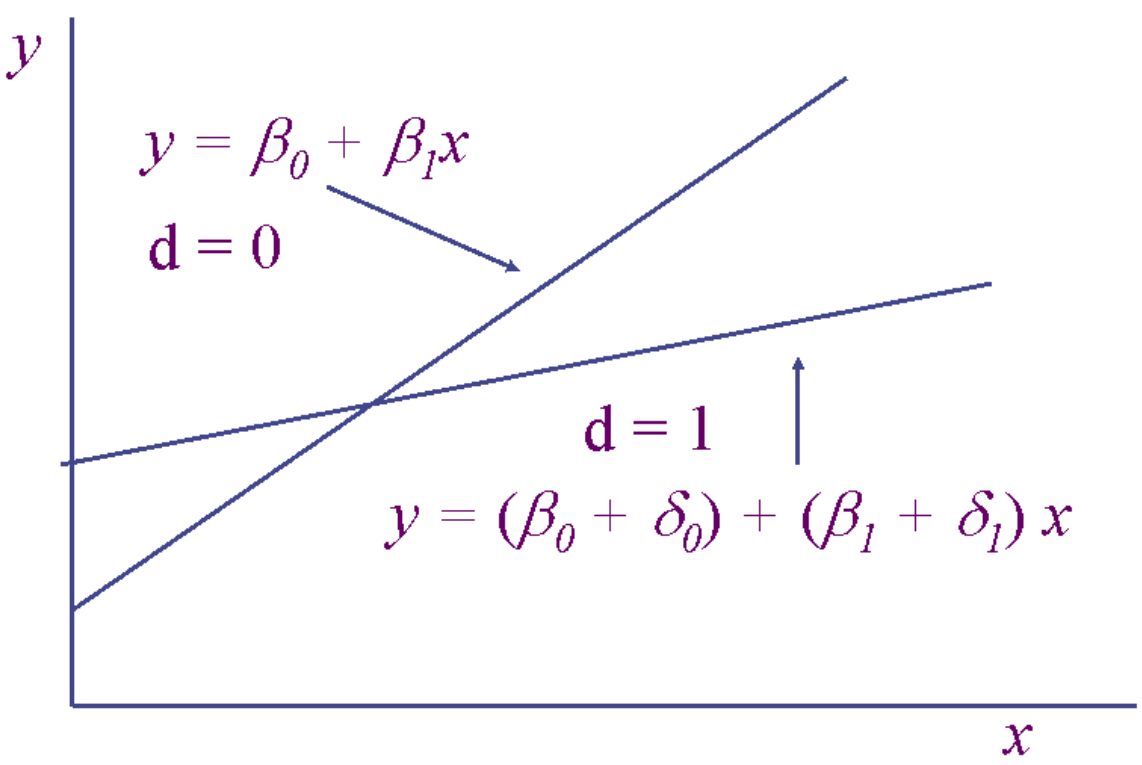
\includegraphics[width = 0.8\linewidth]{fig/dummy2.png}
    		\end{centering}
    	\end{figure}
\end{frame}
%---------------------------------------------------
\begin{frame}[fragile]
	\begin{lstlisting}[language=Stata, numbers=none]
. use datos, clear
. reg bmi Z1 age
	\end{lstlisting}
	\scriptsize{
		\begin{verbatim}
        Source |       SS           df       MS      Number of obs   =     3,278
  -------------+----------------------------------   F(2, 3275)      =     27.72
         Model |  1701.34797         2  850.673984   Prob > F        =    0.0000
      Residual |  100512.889     3,275  30.6909585   R-squared       =    0.0166
  -------------+----------------------------------   Adj R-squared   =    0.0160
         Total |  102214.237     3,277  31.1914059   Root MSE        =    5.5399
  
  ------------------------------------------------------------------------------
           bmi |      Coef.   Std. Err.      t    P>|t|     [95% Conf. Interval]
  -------------+----------------------------------------------------------------
            Z1 |   3.939848   .6174998     6.38   0.000     2.729123    5.150573
           age |  -.0816753   .0218862    -3.73   0.000    -.1245873   -.0387632
         _cons |    29.2826   1.572287    18.62   0.000     26.19984    32.36537
  ------------------------------------------------------------------------------
		\end{verbatim}
	}
\end{frame}
%---------------------------------------------------
\begin{frame}[fragile]
	\begin{lstlisting}[language=Stata, numbers=none]
. use datos, clear
. reg bmi Z1 age mujer
	\end{lstlisting}
	\scriptsize{
		\begin{verbatim}
        Source |       SS           df       MS      Number of obs   =     3,278
  -------------+----------------------------------   F(3, 3274)      =     43.62
         Model |  3928.34017         3  1309.44672   Prob > F        =    0.0000
      Residual |   98285.897     3,274  30.0201274   R-squared       =    0.0384
  -------------+----------------------------------   Adj R-squared   =    0.0376
         Total |  102214.237     3,277  31.1914059   Root MSE        =    5.4791
  
  ------------------------------------------------------------------------------
           bmi |      Coef.   Std. Err.      t    P>|t|     [95% Conf. Interval]
  -------------+----------------------------------------------------------------
            Z1 |   3.768941   .6110363     6.17   0.000     2.570889    4.966993
           age |  -.0778696   .0216502    -3.60   0.000    -.1203189   -.0354204
         mujer |   1.658769   .1925896     8.61   0.000      1.28116    2.036377
         _cons |   28.25224   1.559604    18.12   0.000     25.19434    31.31014
  ------------------------------------------------------------------------------
		\end{verbatim}
	}
\end{frame}
%---------------------------------------------------
\begin{frame}[fragile]
	\begin{lstlisting}[language=Stata, numbers=none]
. use datos, clear
. reg bmi Z1 age mujer mujer_Z1
	\end{lstlisting}
	\scriptsize{
		\begin{verbatim}
        Source |       SS           df       MS      Number of obs   =     3,278
  -------------+----------------------------------   F(4, 3273)      =     33.96
         Model |  4073.37779         4  1018.34445   Prob > F        =    0.0000
      Residual |  98140.8593     3,273   29.984986   R-squared       =    0.0399
  -------------+----------------------------------   Adj R-squared   =    0.0387
         Total |  102214.237     3,277  31.1914059   Root MSE        =    5.4759
  
  ------------------------------------------------------------------------------
           bmi |      Coef.   Std. Err.      t    P>|t|     [95% Conf. Interval]
  -------------+----------------------------------------------------------------
            Z1 |   2.480199   .8463405     2.93   0.003     .8207887     4.13961
           age |  -.0786235   .0216402    -3.63   0.000    -.1210532   -.0361937
         mujer |    1.88688   .2186435     8.63   0.000     1.458188    2.315572
      mujer_Z1 |   2.688477   1.222413     2.20   0.028     .2917055    5.085248
         _cons |      28.19   1.558947    18.08   0.000     25.13339    31.24661
  ------------------------------------------------------------------------------
			
		\end{verbatim}
	}
\end{frame}

%------------------------------------------------------------------------------------
\subsection{Test de Chow o de quiebre estructural}
%------------------------------------------------------------------------------------
\begin{frame}{Test de Chow o de quiebre estructural}
	\begin{itemize}
		\item Probar si una función de regresión es diferente para un grupo versus otro grupo puede ser realizado probando la significancia conjunta
		de las variables dicotómicas y sus interacciones con otras variables.
		\pause
		\item Alternativamente, una manera práctica de verificar que dos grupos tienen funciones de regresión distintas es empleando el test de
		Chow.
		\pause
		\item Bajo este test se calculan tres regresiones y se compuntan la $SCR$ asociados a cada regresión. La primera regresión es la regresión
		empleando todos los datos ($SCR$) y las regresiones restantes son para cada grupo ($SRC_{1}$ y $SRC_{2}$)
		\pause
		\item Con las $SRC$ se computa el estadí­stico $F=\frac{[SCR-(SCR_{1}+SCR_{2})]/(k+1)}{(SCR_{1}+SCR_{2})/(n-2(k+1))}$
	\end{itemize}
\end{frame}